% !TEX root = ../main.tex
\section{Results}\label{sec:results}

% Test was read once on 2026-11-17 (G01_final__grouped). No choice may use it.

\subsection{Main results}\label{sec:main_results}

% Main results on the grouped split. Numbers from experiments/results.jsonl,
% each run's report_test.json and experiments/G01_final__grouped.

\begin{table}[ht]
\centering
\caption{The best model of each family on the grouped split, chosen by
validation accuracy. Single runs, no test-time augmentation, except the final
system. Test was read once, after every choice was made on validation.}
\label{tab:main_results}
\small
\begin{tabular}{@{}llccc@{}}
\toprule
 & & Val & \multicolumn{2}{c}{Test} \\
\cmidrule(l){4-5}
Family & Best model & top-1 (\%) & top-1 (\%) & macro-F1 \\
\midrule
\multicolumn{5}{@{}l}{\textit{Frozen backbones}} \\
Classical classifiers & Logistic regression (D01) & 45.70 & 41.02 & 0.394 \\
Linear probe & VideoMAE-B (P04) & 56.98 & 52.64 & 0.487 \\
Frame temporal head & Transformer (A09) & 70.11 & 69.59 & 0.688 \\
Video backbone, MLP & VideoMAE-B (V07) & 67.18 & 62.74 & 0.619 \\
\multicolumn{5}{@{}l}{\textit{Pose, bat and motion}} \\
Pose alone & Keypoint GRU (E01) & 65.71 & 63.50 & 0.614 \\
Bat, ball, pose & Track fusion (W04) & 70.24 & 68.12 & 0.671 \\
RGB with pose & Late fusion (E03) & 73.49 & 72.59 & 0.719 \\
Motion & Frame differences (W05) & 78.59 & 75.03 & 0.734 \\
\multicolumn{5}{@{}l}{\textit{Fine-tuned end to end}} \\
Original CNN--GRU & EfficientNetV2-S (B01) & 77.69 & 75.23 & 0.731 \\
Image backbone, GRU & ConvNeXt-T (B04) & 81.52 & 79.75 & 0.786 \\
Multi-scale hybrid & F02 & 83.43 & 81.22 & 0.802 \\
Video backbone & MViTv2-S (C06) & 84.51 & 82.13 & 0.819 \\
\midrule
\textbf{Final system} & C06 + F02, flip & \textbf{87.38} & \textbf{84.82} & \textbf{0.843} \\
\bottomrule
\end{tabular}
\end{table}

\begin{table}[ht]
\centering
\caption{The final system and its two members. A single run is the mean and
standard deviation of three seeds, without augmentation. A member with flip
averages its three seeds on the clip and its mirror image.}
\label{tab:final_system}
\begin{tabular}{@{}lccc@{}}
\toprule
 & Val & \multicolumn{2}{c}{Test} \\
\cmidrule(l){3-4}
 & top-1 (\%) & top-1 (\%) & macro-F1 \\
\midrule
MViTv2-S (C06), single run & 85.06 $\pm$ 0.54 & 82.47 $\pm$ 0.39 & -- \\
F02, single run            & 83.39 $\pm$ 0.04 & 80.47 $\pm$ 0.76 & -- \\
\addlinespace
MViTv2-S (C06), 3 seeds with flip & 86.36 & 83.76 & 0.835 \\
F02, 3 seeds with flip            & 85.47 & 82.49 & 0.816 \\
\addlinespace
\textbf{Equal vote of both, with flip} & \textbf{87.38} & \textbf{84.82} & \textbf{0.843} \\
\bottomrule
\end{tabular}
\end{table}


% Written by tools/paper_results.py from every run's reports.
{\small
\setlength{\tabcolsep}{4pt}
\begin{longtable}{@{}llcccc@{}}
\caption{Every experiment: top-1 accuracy (\%) on both splits. Single runs, no test-time augmentation. Test was read once, after the final system was chosen on grouped validation. Runs marked $^{\dagger}$ were repeated with two more seeds (Table~\ref{tab:final_system}); the seed-42 run is shown.}\label{tab:all_results}\\
\toprule
 & & \multicolumn{2}{c}{Author split} & \multicolumn{2}{c}{Grouped split} \\
\cmidrule(lr){3-4}\cmidrule(l){5-6}
ID & Model & Val & Test & Val & Test \\
\midrule
\endfirsthead
\multicolumn{6}{@{}l}{\textit{Table~\ref{tab:all_results}, continued}} \\
\toprule
 & & \multicolumn{2}{c}{Author split} & \multicolumn{2}{c}{Grouped split} \\
\cmidrule(lr){3-4}\cmidrule(l){5-6}
ID & Model & Val & Test & Val & Test \\
\midrule
\endhead
\bottomrule
\endlastfoot
\multicolumn{6}{@{}l}{\textit{Linear probes on frozen features}} \\
P01 & EfficientNetV2-S, ImageNet & 40.66 & 41.09 & 44.42 & 43.40 \\
P02 & ConvNeXt-T, ImageNet & 49.49 & 49.44 & 51.56 & 49.70 \\
P03 & R3D-18, Kinetics-400 & 41.41 & 39.88 & 43.59 & 42.44 \\
P04 & VideoMAE-B, Kinetics-400 & 52.21 & 53.69 & 56.98 & 52.64 \\
P05 & CLIP ViT-B/16 & 39.14 & 38.11 & 42.96 & 44.92 \\
\addlinespace
\multicolumn{6}{@{}l}{\textit{Temporal heads on frozen EfficientNetV2-S frames}} \\
A01 & Mean pooling & 52.78 & 52.13 & 58.19 & 55.18 \\
A02 & Max pooling & 56.19 & 55.82 & 59.27 & 56.40 \\
A03 & GRU-128 (the authors' head) & 51.96 & 50.05 & 54.11 & 52.79 \\
A04 & GRU-64 & 52.53 & 51.11 & 49.52 & 46.55 \\
A05 & BiGRU-128 & 55.93 & 52.68 & 56.15 & 52.89 \\
A06 & LSTM-64 & 47.92 & 46.46 & 52.77 & 49.70 \\
A07 & BiLSTM-64 & 53.09 & 49.90 & 49.78 & 48.88 \\
A08 & Transformer, 2 layers, 4 heads & 66.22 & 65.08 & 68.96 & 67.41 \\
A09 & Transformer, 4 layers, 8 heads & 68.81 & 65.28 & 70.11 & 69.59 \\
A10 & Temporal convolution (TCN) & 67.17 & 66.65 & 69.66 & 66.45 \\
A11 & Attention pooling & 64.90 & 64.02 & 68.13 & 64.97 \\
A12 & NetVLAD & 65.03 & 65.94 & 63.54 & 59.85 \\
A13 & GRU-128, layer-normalised input & 49.43 & 47.17 & 52.71 & 50.25 \\
A14 & GRU-128 on averaged feature maps & 62.44 & 59.26 & 63.10 & 59.24 \\
\addlinespace
\multicolumn{6}{@{}l}{\textit{Classical classifiers on frame-averaged features}} \\
D01 & Logistic regression & 42.49 & 42.16 & 45.70 & 41.02 \\
D02 & SVM, RBF kernel & 34.47 & 36.34 & 40.60 & 39.70 \\
D03 & Random forest & 27.21 & 28.80 & 29.32 & 30.96 \\
D04 & XGBoost & 36.17 & 38.77 & 41.56 & 41.73 \\
D05 & k-nearest neighbours & 18.50 & 19.33 & 23.07 & 22.54 \\
D06 & MLP & 39.39 & 42.51 & 44.17 & 44.01 \\
\addlinespace
\multicolumn{6}{@{}l}{\textit{Frozen backbones with an MLP}} \\
V01 & R3D-18 & 45.58 & 41.80 & 46.91 & 45.69 \\
V02 & MC3-18 & 52.71 & 53.39 & 55.07 & 52.69 \\
V03 & R(2+1)D-18 & 45.90 & 45.80 & 49.59 & 47.61 \\
V04 & S3D & 41.48 & 43.67 & 46.21 & 44.37 \\
V05 & Video Swin-T & 55.74 & 53.39 & 57.43 & 55.53 \\
V06 & MViTv2-S & 51.70 & 51.82 & 54.49 & 52.23 \\
V07 & VideoMAE-B & 61.68 & 61.44 & 67.18 & 62.74 \\
V08 & TimeSformer-B & 50.51 & 54.10 & 57.81 & 54.92 \\
V09 & CLIP ViT-B/16, per frame & 46.46 & 45.24 & 49.71 & 49.70 \\
V10 & DINOv2-B, per frame & 61.36 & 62.45 & 64.18 & 65.94 \\
\addlinespace
\multicolumn{6}{@{}l}{\textit{Image backbones with GRU-128, fine-tuned}} \\
B01 & EfficientNetV2-S (the authors' model) & 79.23 & 78.14 & 77.69 & 75.23 \\
B02 & EfficientNetV2-B3 & 77.02 & 76.82 & 78.84 & 78.48 \\
B03 & Xception & 79.92 & 78.09 & 80.82 & 80.20 \\
B04 & ConvNeXt-T & 80.24 & 80.92 & 81.52 & 79.75 \\
B05 & MobileNetV3-L & 75.00 & 76.06 & 77.76 & 76.09 \\
B06 & ResNet-50 & 77.53 & 76.37 & 80.18 & 77.36 \\
B07 & RegNetY-16GF & 77.90 & 78.04 & 79.67 & 78.17 \\
B08 & Swin-T & 78.41 & 79.30 & 79.54 & 77.01 \\
\addlinespace
\multicolumn{6}{@{}l}{\textit{Video backbones, fine-tuned}} \\
C01 & R(2+1)D-18 & 80.49 & 79.45 & 79.67 & 77.26 \\
C02 & R3D-18 & 78.35 & 77.43 & 79.16 & 77.21 \\
C03 & I3D, ResNet-50 & 77.90 & 76.52 & 80.62 & 78.27 \\
C04$^{\dagger}$ & SlowFast, ResNet-50 & 81.69 & 81.02 & 83.81 & 80.91 \\
C05 & X3D-M & 81.19 & 81.53 & 83.11 & 81.78 \\
C06$^{\dagger}$ & MViTv2-S & 83.40 & 82.79 & 84.51 & 82.13 \\
C07 & Video Swin-T & 81.31 & 79.55 & 82.03 & 79.19 \\
C08 & VideoMAE-B & 80.87 & 81.38 & 82.92 & 82.28 \\
\addlinespace
\multicolumn{6}{@{}l}{\textit{Reproduction of the authors' method}} \\
R01 & Their recipe on their preprocessing & 76.77 & 75.96 & 77.44 & 75.69 \\
R02 & Their recipe on our preprocessing & 79.17 & 79.20 & 78.65 & 79.54 \\
R03 & Our B01 on their preprocessing & 75.44 & 76.01 & 78.14 & 75.89 \\
\addlinespace
\multicolumn{6}{@{}l}{\textit{Pose}} \\
E01 & Keypoints with GRU-128 & 65.72 & 65.49 & 65.71 & 63.50 \\
E02 & ST-GCN on keypoints & 48.67 & 50.61 & 50.86 & 48.27 \\
E03 & A09 and E01, averaged & 72.73 & 71.15 & 73.49 & 72.59 \\
E04 & Cross-attention, pose and RGB & 63.83 & 63.36 & 68.07 & 62.49 \\
\addlinespace
\multicolumn{6}{@{}l}{\textit{Bat, ball and motion}} \\
W01 & Optical flow (RAFT), R3D-18 & 74.18 & 73.43 & 76.04 & 72.79 \\
W02 & Bat track, GRU-128 & 51.01 & 51.67 & 52.84 & 52.54 \\
W03 & Ball track, GRU-128 & 23.30 & 22.22 & 25.81 & 22.44 \\
W04 & Bat, ball and pose tracks & 67.05 & 67.91 & 70.24 & 68.12 \\
W05 & Frame differences, R3D-18 & 75.25 & 74.19 & 78.59 & 75.03 \\
\addlinespace
\multicolumn{6}{@{}l}{\textit{Multi-scale and hybrid}} \\
F01 & B01 with multi-scale features & 76.14 & 76.37 & 78.14 & 75.89 \\
F02$^{\dagger}$ & F01 with a transformer head & 80.68 & 80.11 & 83.43 & 81.22 \\
F03 & C02 and W01, averaged & 79.61 & 79.55 & 80.94 & 79.14 \\
F04 & B01 with a second resolution & 76.58 & 76.47 & 79.60 & 77.66 \\
F05 & B01 with attention over GRU steps & 78.91 & 78.14 & 81.13 & 76.85 \\
\addlinespace
\multicolumn{6}{@{}l}{\textit{Tuning C06, one change each}} \\
T01 & Learning rate $3\times10^{-5}$ & -- & -- & 84.58 & 81.17 \\
T02 & Learning rate $3\times10^{-4}$ & -- & -- & 72.15 & 66.75 \\
T03 & Backbone learning rate $\times0.1$ & -- & -- & 82.54 & 79.14 \\
T04 & Backbone learning rate $\times0.5$ & -- & -- & 85.28 & 80.96 \\
T05 & Label smoothing 0.05 & -- & -- & 85.09 & 82.13 \\
T06 & Label smoothing 0.1 & -- & -- & 85.53 & 82.59 \\
T07$^{\dagger}$ & Class-balanced loss & -- & -- & 85.79 & 82.44 \\
T08 & Stochastic depth 0.4 & -- & -- & 85.15 & 81.98 \\
T09 & Head dropout 0.7 & -- & -- & 84.13 & 81.88 \\
T10 & AdamW, weight decay 0.05 & -- & -- & 85.40 & 81.73 \\
T11 & Colour jitter & -- & -- & 84.32 & 81.27 \\
T12 & Random crop & -- & -- & 84.83 & 82.23 \\
T13 & Time jitter, one frame & -- & -- & 84.51 & 84.16 \\
\addlinespace
\multicolumn{6}{@{}l}{\textit{Tuning F02, one change each}} \\
T14 & Learning rate $3\times10^{-5}$ & -- & -- & 81.26 & 80.10 \\
T15 & Learning rate $3\times10^{-4}$ & -- & -- & 82.54 & 80.30 \\
T16 & Backbone learning rate $\times0.1$ & -- & -- & 79.22 & 77.66 \\
T17 & Backbone learning rate $\times0.5$ & -- & -- & 81.71 & 80.61 \\
T18$^{\dagger}$ & Label smoothing 0.05 & -- & -- & 83.17 & 80.30 \\
T19 & Label smoothing 0.1 & -- & -- & 82.60 & 79.54 \\
T20 & Class-balanced loss & -- & -- & 83.17 & 80.71 \\
T21 & Stochastic depth 0.4 & -- & -- & 83.11 & 81.27 \\
T22 & Head dropout 0.3 & -- & -- & 82.09 & 78.98 \\
T23 & AdamW, weight decay 0.01 & -- & -- & 83.68 & 80.36 \\
T24 & Colour jitter & -- & -- & 82.60 & 81.12 \\
T25 & Random crop & -- & -- & 83.56 & 80.46 \\
T26 & Time jitter, one frame & -- & -- & 82.92 & 81.27 \\
T27$^{\dagger}$ & 20 frames instead of 15 & -- & -- & 83.94 & 80.20 \\
\addlinespace
\midrule
G01 & \textbf{Final: C06 + F02, 3 seeds, flip} & -- & -- & \textbf{87.38} & \textbf{84.82} \\
\end{longtable}
}


\subsection{Metrics}

% Accuracy, macro-F1, per-class recall (equations).

\subsection{Frame models}

\subsection{Video models}

\subsection{Pose and bat tracks}

\subsection{Tuning (Family T)}

\subsection{Ensemble}

\subsection{Error analysis}

% Most common mistakes on test (true -> predicted): Lofted Offside -> Lofted
% Legside 22, Pull -> Hook 19, Hook -> Pull 19, Down The Wicket -> Lofted
% Offside 14, Lofted Legside -> Lofted Offside 12, Upper Cut -> Square Cut 10.
% All are neighbouring shots; Grad-CAM shows the same pairs.

\input{tables/tab_per_class}

\begin{figure}[ht]
  \centering
  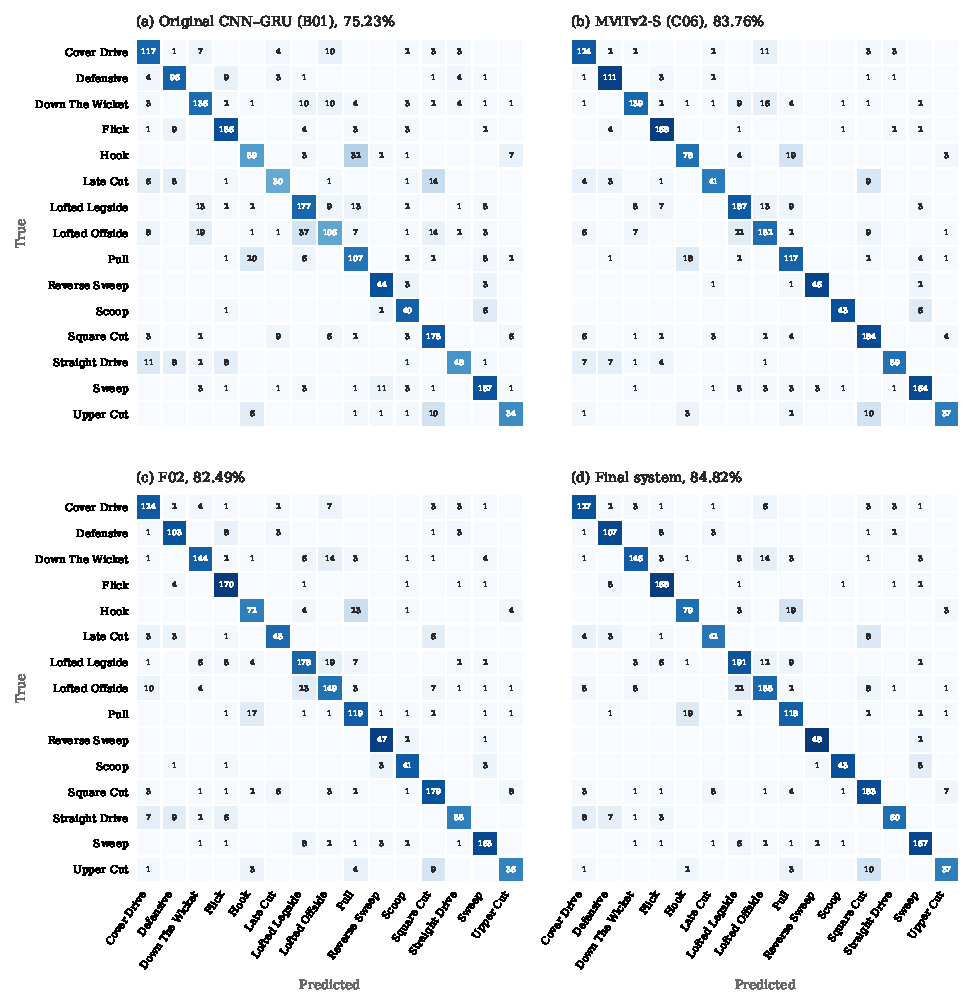
\includegraphics[width=\textwidth]{fig_confusion_members.pdf}
  \caption{Confusion matrices on the grouped test set (1,970 clips), from the
  original CNN--GRU to the final system. (a) B01, one run. (b, c) The two
  members, each as it votes: three seeds averaged on the clip and its mirror
  image. (d) Their equal vote. Numbers are clip counts; the shade is the share
  of each true class, so small classes read on the same scale.}
  \label{fig:confusion}
\end{figure}
